% Artyom Voronin
%     _                     
% ___| |__  _ __  _ __ ___  
%/ __| '_ \| '_ \| '_ ` _ \ 
%\__ \ |_) | |_) | | | | | |
%|___/_.__/| .__/|_| |_| |_|
%          |_|              
%
% Brno, 2021

\documentclass[class=article, crop=false]{standalone}
\usepackage[subpreambles=true]{standalone}
\usepackage{subcaption}

\usepackage{sectsty}
\usepackage{graphicx}
\graphicspath{{img/}{../img/}{../../img/}}
\usepackage{listings}
\lstset{language=Matlab}
\usepackage{hyperref}
\usepackage{amsmath}
\usepackage{import}
\usepackage{subfiles}
\usepackage{caption}
\usepackage[utf8]{inputenc}
\usepackage[english]{babel}

%\usepackage[square, numbers]{natbib}
%\bibliographystyle{unsrtnat}
%\usepackage[nottoc]{tocbibind}

\topmargin=-0.45in
\evensidemargin=0in
\oddsidemargin=0in
\textwidth=6.5in
\textheight=9.0in
\headsep=0.25in

%\title{Preprocessing data from pneumatic actuator}
%\author{Artyom Voronin} 
%\date{}

\begin{document}
\section{Preprocessing measured data}

\subsection{Data overview}

Data has been collect from 8 types of sensors:

\begin{itemize}
\item Flow sensor
\item Microphones
\item Pressure sensor
\item Strain gauge
\item Position encoder
\item Accelerometer
\item Temperature sensor
\item Proximity sensor
\end{itemize}

Data has been accumulated to ".mat" files.
Each file contains signals from sensors during 10 seconds measurements with
different pneumatic actuator configuration. Example results from one
experiment are represented in figures \ref{fig:data_exmp1},
\ref{fig:data_exmp2}. Data files have been reshaped
to Data Ensembles format used for Condition monitoring purposes. This
format allows processing data without copying the whole dataset to
memory at once but processes them one by one. In large datasets it gives an
option to manipulate with data without problems with memory.

\begin{figure}[h!]
    \centering
    \begin{subfigure}{.5\textwidth}
        \centering
        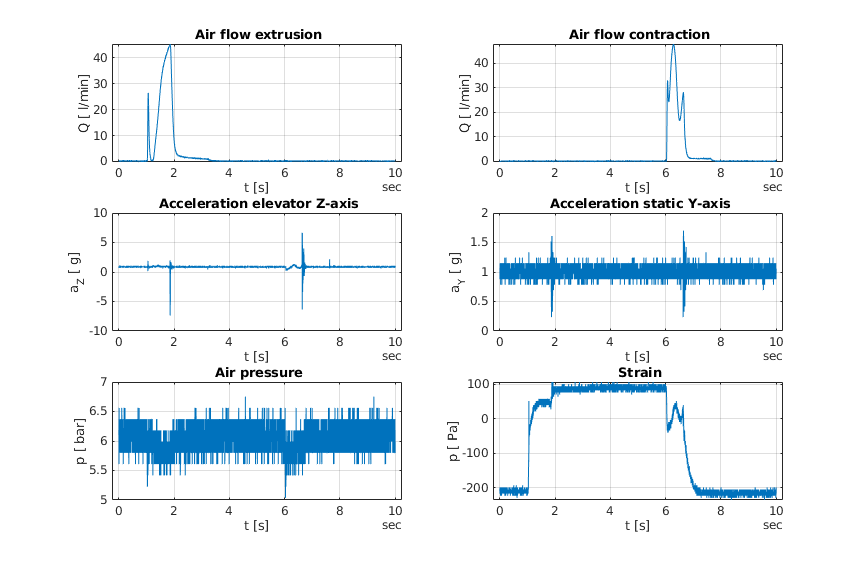
\includegraphics[width=1.1\textwidth]{data_example1.png}
    \end{subfigure}%
    \begin{subfigure}{.5\textwidth}
        \centering
        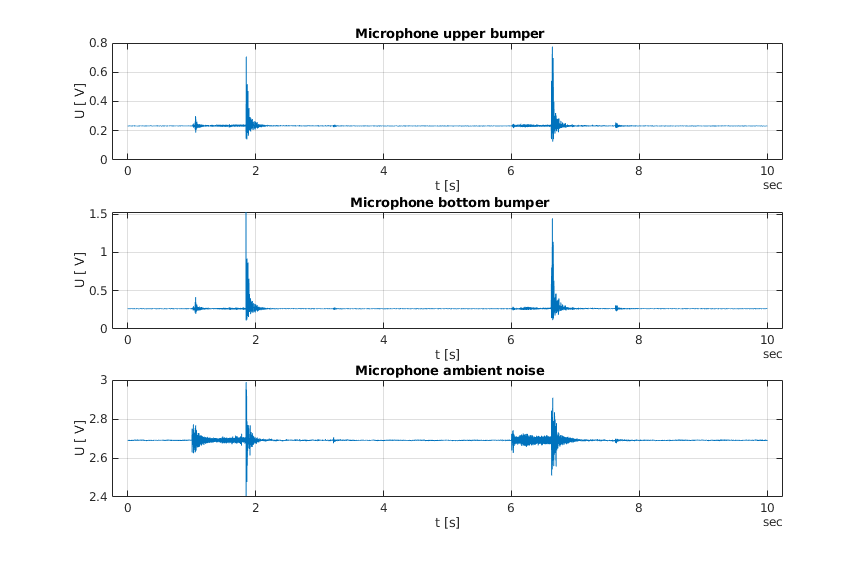
\includegraphics[width=1.1\textwidth]{data_example2.png}
    \end{subfigure}
    \caption{Example of measured data \#1}
    \label{fig:data_exmp1}
\end{figure}

\begin{figure}
    \centering    
    \begin{subfigure}{.5\textwidth}
        \centering
        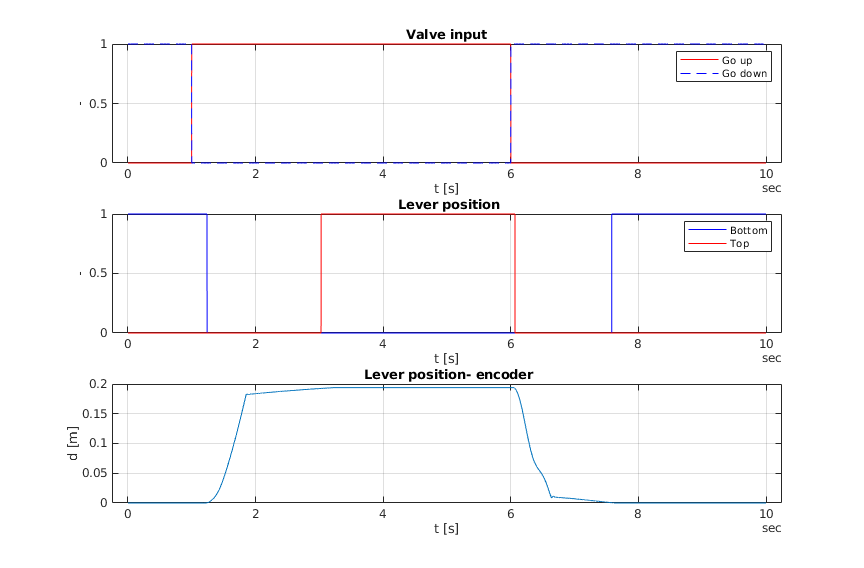
\includegraphics[width=1.1\textwidth]{data_example3.png}
        \caption{Example of measured data}
    \end{subfigure}%
    \begin{subfigure}{.5\textwidth}
        \centering
        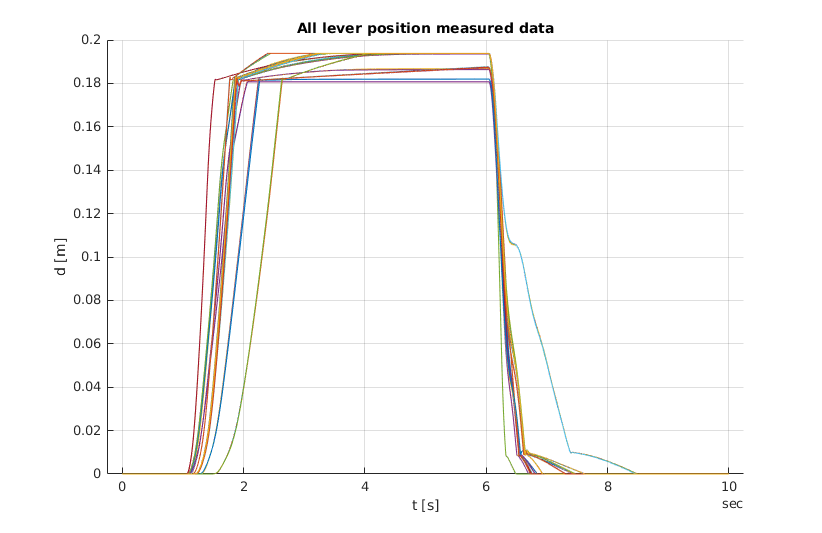
\includegraphics[width=1.1\textwidth]{lever_positions.png}
        \caption{Example of all measured lever positions}
    \end{subfigure}
    \caption{Example of measured data \#2}
    \label{fig:data_exmp2}
\end{figure}

\subsection{Preprocessing}
Measured signals require preprocessing for feature extraction. Signals were
filtered and preprocessed concerning the preservation of the information
base. Filters were design concerning Amplitude-frequency response for
particular signals, using Fast-Fourier transformation. For smoothing
data Moving Average function were used.
As an example, the figure \ref{fig:preprocess} is shown the "raw" and filtered signals.
The whole dataset of preprocessed data is relatively big. For
time-saving, parallel computing was used for all computationally
demanding parts of the code.

\begin{figure}[h!]
    \centering
    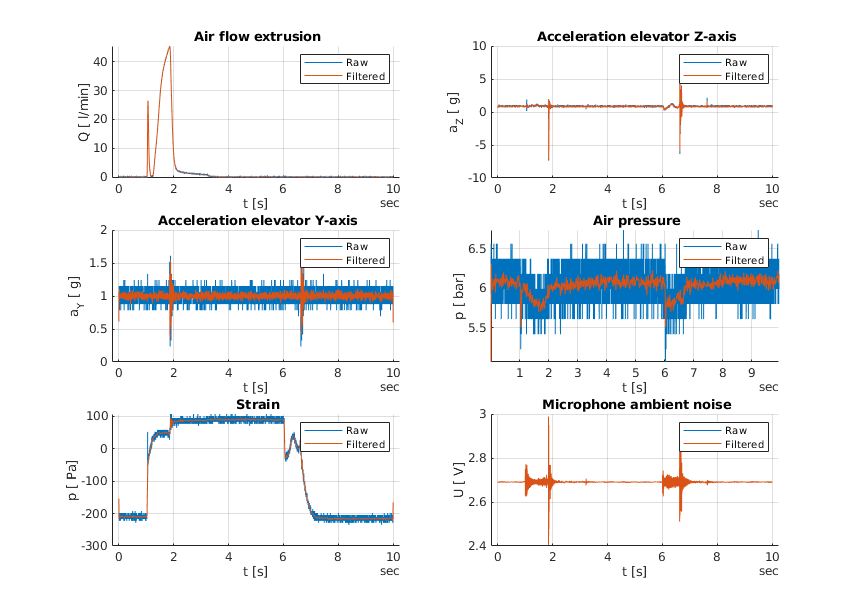
\includegraphics[width=0.8\textwidth]{preprocessed_data.png}
    \caption{Example of measured data after filtration}
    \label{fig:preprocess}
\end{figure}


\subsection{Feature extraction}

For classification task purpose from the signals have been extracted
statistical features such as mean, median, peak to peak value, etc.
As a condition "FaultCode" variable
were used. This variable represent configuration of pneumatic actuator
during the measurement.

All calculated features were added to the dataset and were ranked by
Kruskal-Wallis ANOVA algorithm. Following table \ref{tab:feat} contain
5 first best features ranked for classification purpose.

\begin{table}[h]
    \centering
    \begin{tabular}{|c|c|c|}
        \hline
        1. & LeverPosition\_Stat\_Var & Lever position variance \\
        2. & StrainGauge\_Stat\_Mean  & Strain gauge mean value \\
        3. & StrainGauge\_Stat\_Skewness  & Strain gauge Skewness value \\
        4. & LeverPosition\_Stat\_RMS  & Lever position Root mean square
        level \\
        5. & LeverPosition\_Stat\_mean  & Lever position mean value \\ 
        \hline
    \end{tabular}
    \caption{First 5 ranked features}
    \label{tab:feat}
\end{table}


\subsection{Classification task}

The main goal of the classification task is to train a model that can
predict the "FaultCode" of pneumatic actuator configuration by
calculated features.
Respecting to table \ref{feat}, the first five features have been used to
find the best classification model for our data.
Principal component analysis (PCA) has been used to reduce the number of
features and chose the best representants.
The trained model has been exported to
\textbf{models/} directory.
The confusion matrix of the trained classification model shown in figure
\ref{fig:conf}. Model accuracy on validation data is $\approx 93 \%$
\ref{fig:pred}.

\begin{figure}[h!]
    \centering    
    \begin{subfigure}{.5\textwidth}
        \centering
        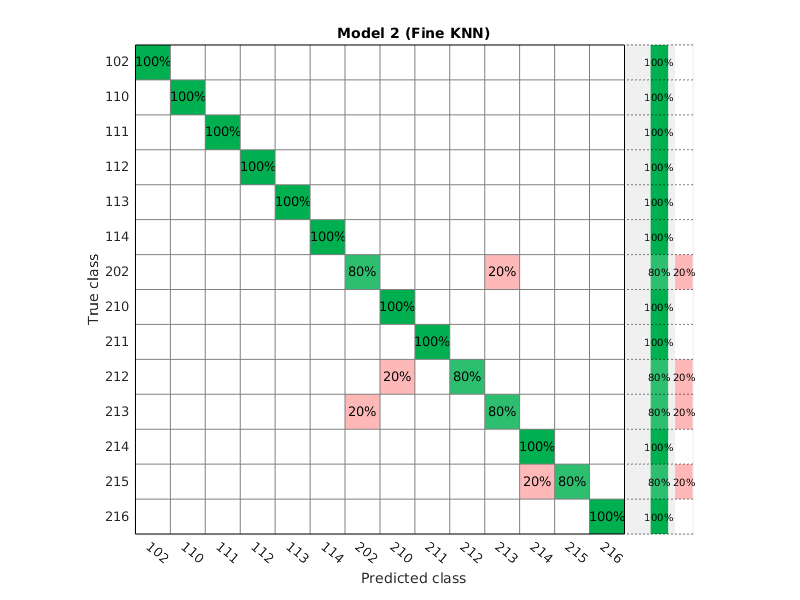
\includegraphics[width=1.1\textwidth]{conf_matrix_kw_ranked.png}
        \caption{Confusion matrix of the model}
        \label{fig:conf}
    \end{subfigure}%
    \begin{subfigure}{.5\textwidth}
        \centering
        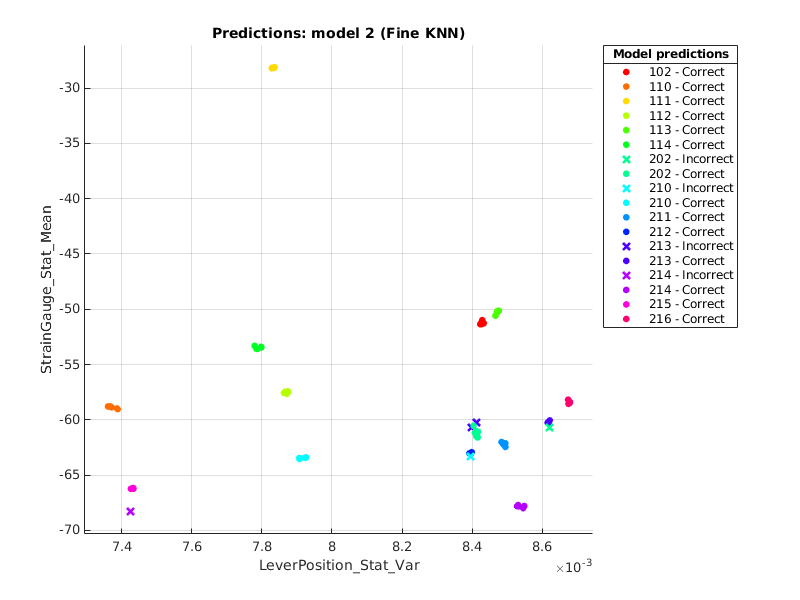
\includegraphics[width=1.1\textwidth]{model_kw_ranked_pca.png}
        \caption{Model predictions}
        \label{fig:pred}
    \end{subfigure}
    \caption{Trained model performance}
    \label{model}
\end{figure}



%\subsection{Conclusion}
%Measured data from the pneumatic actuator were preprocessed and used for
%feature extraction. For faster processing, the code has been modified to
%parallel computing. A classification model was trained to predict the
%"FaultCode" variable, which indicates the current configuration of the
%pneumatic actuator. The best results achieve with two first features from
%table \ref{tab:feat}.
%Measured data from the pneumatic actuator were preprocessed and used for
%feature extraction. For faster processing, the code has been modified to
%parallel computing. A classification model was trained to predict the
%"FaultCode" variable, which indicates the current configuration of the
%pneumatic actuator.

%\pagebreak
%\subsection{Appendix}
%
%\subsubsection{Project structure:}
%\begin{lstlisting}
%* app_sessions     % Saved Feature Designer app sessions
%* data_converted/  % Converted, preprocessed data
%* data_original/   % Raw data from sensors
%* data_test/       % For test purpose only
%* dataset/         % Dataset feature table for Classification
%* doc/             % Documentation for the project
%* legacy/          % Legacy scripts
%* models/          % Saved model, training script
%* scripts/         % All functions used in the project
%* main.m           % Main script
%
%\end{lstlisting}
%
\subsubsection{Libraries and Toolboxes:}

\begin{itemize}
\item Signal Processing Toolbox 
\item Predictive Maintenance Toolbox 
\item Diagnostic Feature Designer 
\item Classification Toolbox 
\end{itemize}

\end{document}
